\documentclass[11pt,american,czech,oneside]{book}
    \usepackage[a4paper]{geometry}

    \usepackage[T1]{fontenc}
    \usepackage[utf8]{inputenc}
    \usepackage{babel}
    \usepackage{amsmath,amssymb,amsfonts,amsthm}
    \usepackage{indentfirst}
    \usepackage{graphicx}
    \usepackage[boxed]{algorithm2e}
    \SetKwArray{Marker}{marker}

    \usepackage{tikz}
    \usepackage{caption,lipsum}
    \usepackage{listings}
    \usepackage{mathtools}
    \usepackage{multirow}
    \usepackage{url}
    \usetikzlibrary{calc}
    \setcounter{secnumdepth}{3}

\theoremstyle{plain}
    \newtheorem{theorem}{Věta}
    \newtheorem{lemma}{Lemma}
    \newtheorem{proposition}{Tvrzení}
    \newtheorem*{corollary}{Důsledek}
\theoremstyle{definition}
    \newtheorem{definition}{Definice}
    \newtheorem{remark}{Poznámka}
    \newtheorem{example}{Příklad}
    \newtheorem{observation}{Pozorování}
\renewcommand*{\proofname}{Důkaz}

\DeclarePairedDelimiter\floor{\lfloor}{\rfloor}

%\newcommand{\TODO}[1]{\textcolor{red}{TODO: #1}\PackageWarning{TODO:}{TODO: #1!}}
\newcommand{\TODO}[1]{\textcolor{red}{TODO: #1}}

\begin{document}

%----------------------------------------------------------------------

\chapter{Grafy, stromy} \TODO{nejaky hezky obrazky?} 
V této kapitole definujeme graf jakožto matematickou strukturu, popíšeme základní pojmy týkající se grafů a nastíníme možné vztahy mezi grafem a maticí. Dále definujeme strom, jakožto speciální případ grafu. Terminologie je převzata z \cite{koub:11}

\section{Základní grafová terminologie}

\begin{definition}
  Mějme množinu $V$ a množinu $E = \left\{ \left\{ u,v \right\} | u,v \in V \right\}$. Uspořádanou dvojici $G := (V,E)$, nazveme neorientovaný graf. Množinu $V$ nazýváme množinou vrcholů grafu $G$, jejím prvkům říkáme vrcholy, množinu $E$ nazýváme množinou hran grafu $G$, jejím prvkům říkáme hrany. Prvky hrany $e$ označujeme jako vrcholy incidentní hraně $e$ nebo koncové body hrany $e$. Říkáme, že hrana $e = \{v,w\}$ spojuje vrcholy $v$ a $w$.
\end{definition}

Pokud neuvažujeme hrany jako nejvýše dvouprvkové množiny vrcholů, ale  jako uspořádané dvojice $(u,v)$, nazýváme odpovídající graf \textbf{orientovaný}. Obvykle uvažujeme orientované a neorientované grafy zvlášť, ale je možné uvažovat i jejich kombinaci. Graf, v němž se vyskytují jak orientované tak neorientované hrany, nazýváme \textbf{smíšený}. Řekneme, že neorientovaný graf $G$ je \textbf{úplný}, pokud $\forall u, v \in V$ $\left(\{u,v\} \in E\right)$.

Povšimněme si, že v definici grafu není vyloučen případ, kdy jsou oba koncové body hrany shodné. Hrana je pak jednoprvkovou množinou a nazýváme ji \textbf{smyčkou} v grafu.

\begin{remark}
  V neorientovaném grafu $G=(V,E)$ platí, že jeho množina hran $E$ je podmnožinou ${V \choose 2} \cup V$, kde $V \choose 2$ značí množinu všech dvouprvkových podmnožin množiny $V$. V orientovaném grafu $H=(W,F)$ je $F$ podmnožinou množiny $W \times W$, tj. všech uspořádaných dvojic vrcholů z $W$.
\end{remark}

\textbf{Stupněm vrcholu} $v \in V$ rozumíme počet vrcholů spojených s vrcholem $v$, značíme $d(v)$. Množinu všech vrcholů, které jsou v grafu $G$ spojeny s vrcholem $v$ značíme $\mathrm{adj}_G(v)$. Pokud je z kontextu jasné o jaký graf se jedná, dolní index vynecháváme.

\begin{definition}
  \textbf{Podgrafem} grafu $G$ nazveme libovolný graf $H=(W,F)$ který splňuje: $W\subseteq V$, $F\subseteq E$ a všechny vrcholy incidentní hranám z $F$ náleží do $W$. Úplný podgraf grafu $G$ nazýváme \textbf{klikou} v grafu $G$. Podgrafem grafu $G$ \textbf{indukovaným} množinou vrcholů $W$ nazveme takový podgraf $G$, který obsahuje všechny hrany grafu $G$, jejichž oba koncové body náleží do $W$, značíme $G(W)$.
\end{definition}

\begin{definition}
  Mějme graf $G=(V,E)$ a zobrazení $\omega:V \rightarrow \mathbb{R}$, resp. $c: E \rightarrow \mathbb{R}$. Přidáním zobrazení $\omega$, resp. $c$ ke~grafu $G$ dostaneme graf, který nazýváme \textbf{ohodnocený}, resp. \textbf{vážený} reálným ohodnocením.
\end{definition}

\begin{definition}
  Mějme neorientovaný graf $G=(V,E)$, nechť $k$ je přirozené číslo. Posloupnost vrcholů $(v_i)_{i=1}^{k}$ nazveme \textbf{sledem} v grafu $G$, pokud $\forall i \in \{1,...,k\} (\{v_{i-1},v_i\} \in E)$. Pokud navíc  $\forall i,j \in \{1,...,k\} (i \neq j \Rightarrow v_i \neq v_j)$, nazveme posloupnost $(v_i)_{i=1}^{k}$ \textbf{cestou}.
\end{definition}

Existuje-li mezi libovolnými dvěma vrcholy grafu cesta, řekneme, že graf je \textbf{souvislý}.
\textbf{Vzdáleností} dvou vrcholů v souvislém grafu $G=(V,E)$ nazveme délku nejkratší cesty mezi těmito dvěma vrcholy. Vzdáleností vrcholu $v \in V$ od množiny vrcholů $W \subset V$ nazveme minimální vzdálenost mezi vrcholem $v$ a libovolným vrcholem náležícím do $W$. 

\medskip

Při používání víceúrovňových metod dělení grafů (viz kapitola \ref{multilevel}) budeme často odvozovat z grafu jiný graf shluknutím množin jeho vrcholů Takový graf budeme nazývat faktorgraf a formálně jej definujeme následovně.
\TODO{n}
\begin{definition}
  Nechť $\mathcal{P} = \{P_1,\ldots,P_n\}$ je rozkladem množiny vrcholů $V$ grafu $G = (V, E)$ a $|V|=n$. Faktorgrafem grafu $G$ nazveme graf $G / \mathcal{P} = (\mathcal{P}, \mathcal{E_P})$, kde 
  \[
    \left(
      (P_i, P_j)\in \mathcal{E_P} \mbox{ pro } i,j \in \{1,\ldots,n\}, i \neq j 
    \right)
    \Leftrightarrow {P_i \cap \mathrm{adj}_G(P_j) \neq \emptyset}
    .
  \]
\end{definition}

Proces vytváření faktorgrafu $G / \mathcal{P}$ z grafu $G$ je znázorněn na obrázku \ref{faktorgrafImg}

\bigskip
{
  \centering
  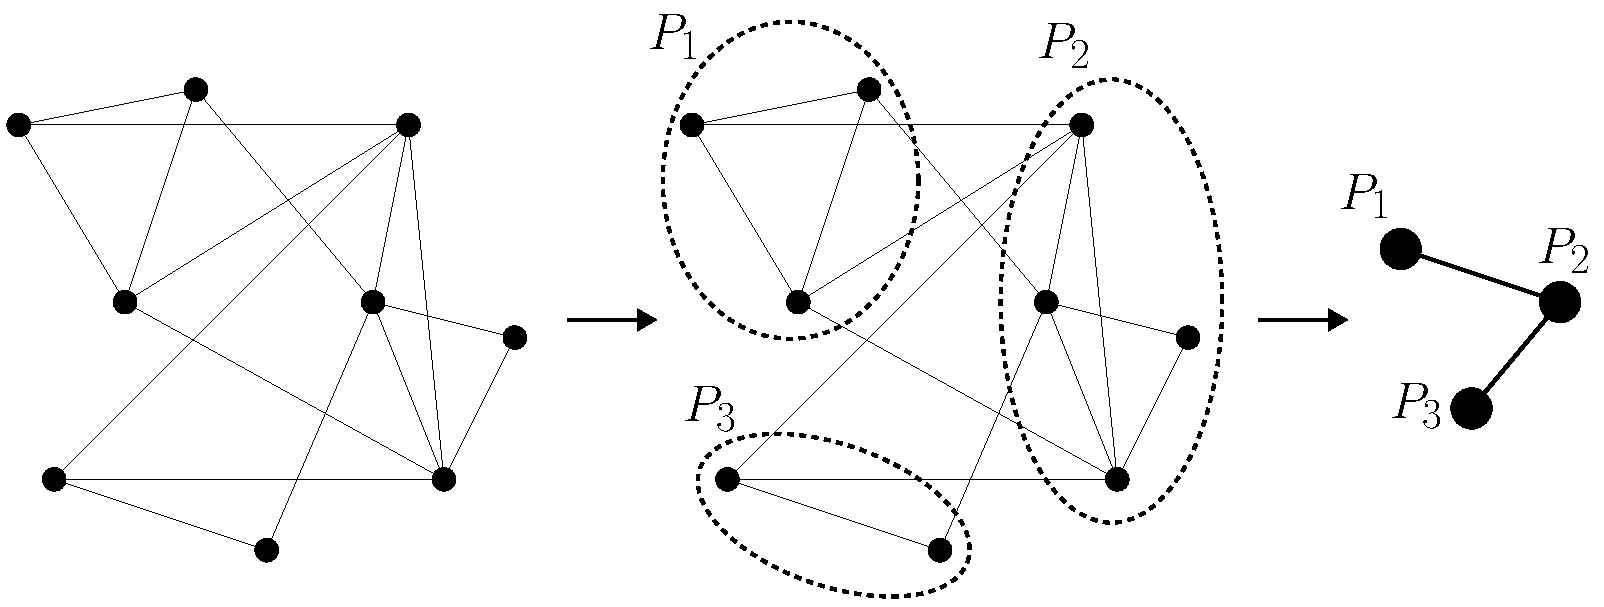
\includegraphics[width=0.8\textwidth]{pictures/faktorgrafcomplete.pdf}
  \captionof{figure}{Proces vytváření faktorgrafu \label{faktorgrafImg}}
}

\TODO{potrebuju ctvercovou sit? Kdyz budu delat ND, tak jo}

\section{Strom}

Nyní zaveďme základní pojmy týkající speciální třídy grafů nazývané stromy \cite{koub:11}

\begin{definition}
  \textbf{Stromem} $T=(V,E)$ nazveme konečný souvislý neorientovaný graf bez cyklů. Pokud navíc v grafu $T$ vyznačíme bod $r \in V$, nazýváme uspořádanou dvojici $(T,r)$ \textbf{kořenovým stromem} a bod $r$ nazveme kořenem tohoto stromu.
\end{definition}

Z definice stromu je patrné, že každý vrchol $v$ kořenového stromu $(T,r)$ spojuje s kořenem tohoto stromu právě jedna cesta.
Vrcholy ležící na této cestě nazveme \textbf{předchůdci} vrcholu $v$. Předchůdce vrcholu $v$ různé od $v$ nazýváme \textbf{vlastními předchůdci} vrcholu $v$. Vrcholy, jejichž předchůdcem je vrchol $v$, nazýváme \textbf{následníky} vrcholu $v$. Vrcholy bez následníků nazýváme \textbf{listy stromu} $T$, vrcholy alespoň s jedním následníkem nazýváme \textbf{vnitřní vrcholy} stromu $T$.

\begin{definition}
  \textbf{Podstromem} stromu $T$ určeným vrcholem $v$ nazveme podgraf stromu $T$ indukovaný vrcholem $v$ a a všemi jeho následníky.
\end{definition}

\section{Vztah grafu a matice}
\label{GrMatRel}
Grafy a matice spolu úzce souvisí, což nám umožňuje převádět problémy na maticích na problémy na grafech a naopak. Nezanedbatelným praktickým důsledkem jejich vzájemného vztahu je i možnost používat grafové algoritmy při řešení některých maticových úloh, především může být tento přístup výhodný pro řídké matice. Dělení grafů může posloužit například při snaze o paralelizaci rozkladu matice.

Uvažujme neorientovaný graf $G=(V,E)$ s vrcholy $V = \{v_1, \ldots, v_n\}$ a hranami $E = \{e_1, \ldots, e_m\}$. Tento graf lze reprezentovat pomocí matice dvěma základními způsoby. \textbf{Maticí sousednosti} grafu $G$, neboli adjacenční maticí, nazveme matici $A_G$ o rozměrech $n \times n$, jejíž prvek na pozici $(i,j)$ je definován jako:
\[
  {(A_G)}_{i,j} :=
  \left\{
    \begin{array}{@{\,}ll}
      1  & \mbox{existuje-li hrana spojující vrcholy $v_i, v_j$} \\
      0  & \mbox{jinak}
    \end{array}
  \right.
\]

 \textbf{Maticí incidence} grafu $G$ nazveme matici o rozměrech $n \times m$  definovanou následovně:
\[
  {(\bar{A}_G)}_{i,j} :=
  \left\{
	  \begin{array}{@{\,}ll}
		  1  & \mbox{je-li $v_i$ koncovým vrcholem hrany $e_j$} \\
		  0  & \mbox{jinak}
	  \end{array}
  \right.
\]

V kapitole \ref{spektral} budeme potřebovat \textbf{Laplaceovu matici} $Q$ grafu $G$. Jedná se o matici o rozměrech $n \times n$ definovanou následovně:
\[
Q_{ij} :=
\left\{
	\begin{array}{@{\,}ll}
		-1  & \mbox{pro } i \neq j, (v_i,v_j) \in E \\
		0 & \mbox{pro } i \neq j, (v_i,v_j) \notin E\\
        d(i) & \mbox{pro } i = j
	\end{array}
\right.
\]
Laplaceovu matici $Q$ lze tedy vyjádřit jako $Q = D - A_G$, kde $D$  značí diagonální matici se stupni jednotlivých vrcholů na diagonále.

\medskip

Pokud chceme reprezentovat matici pomocí grafu, většinou nám stačí zachytit její strukturu. V takovém případě můžeme pro popis obecně nesymetrické matice $A$ o rozměrech $n \times n$ použít orientovaný graf s množinou vrcholů $V = {v_1,\ldots,v_n}$ a množinou hran $E =\left\{(v_i,v_j) \ | \ a_{ij}\neq 0\right\}$. V případě, že je matice $A$ symetrická, můžeme ji analogickým způsobem reprezentovat pomocí neorientovaného grafu.
Pokud bychom chtěli do grafu zanést i numerické hodnoty jednotlivých prvků matice, museli bychom použít ohodnocený graf.

\begin{remark}
  Pro jednoduchost zaveďme následující terminologii. Říkáme, že graf $G$ \textbf{odpovídá} matici $A$ právě tehdy, když matice $A$ má nenulové prvky na stejných pozicích jako matice sousednosti grafu $G$.
\end{remark}

\bigskip
{
  \label{MatGrPicture}
  \centering
  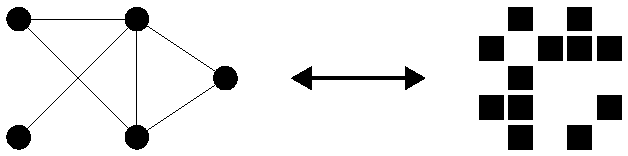
\includegraphics[width=0.7\textwidth]{pictures/matgr.pdf}
  \captionof{figure}{Příklad grafu a jemu odpovídající struktury matice\label{prGrMat}}
}
\bigskip

Pro reprezentaci ne nutně čtvercové matice $A$ o rozměrech $m\times n$ můžeme také použít bipartitní graf, který je definován následovně:

\begin{definition}
  Graf $G=(V,E)$ nazveme bipartitním, pokud existuje rozklad množiny $V$ na podmnožiny $R$, $B$ takové, že ${R \choose 2} \cap E = {B \choose 2} \cap E = \emptyset$.
\end{definition}

Jinými slovy se jedná o graf, který lze rozdělit na dvě části tak, že v žádné z částí není ani jedna hrana. Takovýto bipartitní graf se standardně značí $G=(R,B,E)$ a pokud za jeho pomoci chceme reprezentovat matici $A$, pokládáme $|R|=m$, $|B|=n$ a $E = \left\{(v_i,v_j) \ | \ v_i \in R, v_j \in B, a_{ij} \neq 0 \right\}$.

\TODO{Příklad = obrázek}

%----------------------------------------------------------------------

\chapter{Dělení grafů}

V této kapitole formálně popíšeme problém dělení grafu na $k$ podgrafů a definujeme pojmy s ním spojené. Vzhledem k tomu, že v naší implementaci používáme pro dělení grafů profesionální softwarovou knihovnu METIS \cite{kary:13}, zaměříme se nejprve na schéma víceúrovňového dělení grafu jakožto algoritmus používaný při profesionálních implementacích dělení grafů. Dále se budeme věnovat některým technikám, které tvoří součást víceúrovňového dělení grafů, konkrétně spektrálnímu dělení grafu a vylepšovacímu algoritmu podle Kernighana a Lina \cite{keli:70}. \TODO{Doresit ND}Na závěr kapitoly zmíníme algoritmus metody vnořených řezů (Nested Dissection) jakožto konkrétní příklad víceúrovňového algoritmu pro dělení grafů \TODO{zdroj}.

Dělení grafů na $k$ podgrafů je praktický problém s bohatým teoretickým zázemím a mnoha aplikacemi. Může nám pomoci při řešení parciálních diferenciálních rovnic na moderních počítačových architekturách \cite{posl:90} a nezanedbatelnou roli hraje také při výrobě mikroprocesorů metodou VLSI nebo při řešení velkých systémů lineárních rovnic \cite{keli:70, pis:84}. Často dochází k omezení se na dělení grafu na dva podgrafy, v této práce se však pokusíme prozkoumat i dělení grafu na více částí.

Podmínky, které jsou na výsledné rozdělení grafu kladeny, se mohou lišit v závislosti na daném použití. V této kapitole popíšeme klasická kritéria, která se používají pro určování kvality rozdělení grafu, v kapitole \ref{dalsiParametry} poté bude popsán problém dělení grafů vzhledem k dodatečným kritériím s důrazem na rozklady matic.

\section{Formální definice dělení grafu}

Jako dělení grafu na $k$ částí označujeme hledání rozkladu množiny vrcholů tohoto grafu na $k$ podmnožin. V nejklasičtějším případě je problém dělení grafů na $k$ podgrafů definován následovně.
\begin{definition}
  Mějme graf $G=(V,E)$, $|V| = n$. \textbf{Rozdělením grafu} $G$ na $k$ podgrafů nazveme rozklad množiny vrcholů $V$ na vzájemně disjunktní podmnožiny $V_1, V_2, \ldots, V_k$.   
\end{definition}

\begin{remark}
  Rozdělení grafu běžně zapisujeme jako vektor $P$ o délce $n$ takový, že pro každý vrchol $v_i \in V$ je index podgrafu, v němž se vrchol v nachází, určen $i$-tou složkou vektoru $P$.  
\end{remark}

Řekneme, že rozdělení je \textbf{optimální} vzhledem k základním kritériím, pokud splňuje:
\begin{enumerate}
  \item $\forall i \in \{1, \ldots, k \} \ |V_i|=n/k$
  \item Počet hran spojujících vrcholy ležící v různých podmnožinách je minimální možný.
\end{enumerate}

Pokud má graf $G$ sudý počet vrcholů a rozdělíme ho na dvě části s množinami vrcholů $V_1, V_2$, které mají stejný počet prvků, nazveme toto rozdělení \textbf{bisekcí} a velikost hranového separátoru nazýváme \textbf{šířkou bisekce}.

Mějme graf $G=(V,E)$ a jeho rozdělení na $k$ podgrafů s množinami vrcholů $V_1, V_2, \ldots, V_k$. Množinu hran, jejichž jeden koncový bod náleží do $V_i$ a druhý do $V_j$ pro $i \neq j$ nazveme \textbf{hranovým separátorem}, značíme $\delta(V_1,\ldots,V_k)$. Jinou variantou je hledat rozdělení grafu pomocí vrcholového separátoru.
\textbf{Vrcholovým separátorem} $S_G$ grafu $G$ nazveme podmnožinu množiny vrcholů $V$ takovou, že odstraněním všech vrcholů náležících do $S_G$ z grafu $G$ dojde k jeho rozpadu na nejméně $k$ komponent odpovídajících jednotlivým částem rozdělení. Řešení problému optimální transformace mezi hranovým a vrcholovým separátorem, známe-li jeden z nich, můžeme naleznout v \cite{pofa:90}. To nám ale nic neříká o řešení problému nalezení optimálního hranového nebo vrcholového separátoru \cite{liu:89}.

Ukazuje se, že rozhodovací problém pro optimální rozdělení grafu je NP-úplný \cite{gajo:79}. Existují však algoritmy, které rozdělí graf v rozumném čase, přičemž kvalita jimi nalezeného rozdělení bude poměrně dobrá \cite{lita:79}.

\section{Obecné schéma víceúrovňového dělení grafů}
\label{multilevel}

Víceúrovňové dělení grafů slouží k převedení problému dělení grafu s velkým počtem vrcholů na problém dělení grafu s počtem vrcholů výrazně menším. Tím může dojít k výraznému zkrácení času potřebného pro celkovou dobu běhu algoritmu \TODO{zdroj}, proto je tento postup využíván v profesionálních softwarových nástrojích pro dělení grafů \cite{lehe:95, kary:13}. Nejobecnější popis tohoto schématu sestává ze tří základních fází: zhrubovací fáze (coarsening phase), rozdělení vzniklého grafu a projekce tohoto rozdělení zpět na původní graf (refinement phase).

\paragraph{Zhrubovací fáze}
Základní myšlenkou zhrubovací fáze víceúrovňového schématu dělení grafů je vytvořit z původního grafu $G$ graf $G_m$ s menším počtem vrcholů. Jinými slovy jde o konstrukci posloupnosti grafů $(G_i)_0^m$ takové, že $G_0 := G$ a pro každé dva po sobě jdoucí členy této posloupnosti platí, že $G_{i+1}$ je faktorgrafem $G_i$ s menším počtem vrcholů. 

Pro konstrukci posloupnosti $(G_i)_0^m$ existuje několik možných postupů \cite{kaku:98} \TODO{zdroje? kaku je souhrn}. Ve většině schémat pro tvorbu grafu s méně vrcholy jsou podmnožiny množiny vrcholů grafu $G_i$ spojovány v jeden vrchol, čímž vznikne hrubší graf $G_{i+1}$ splňující výše uvedené podmínky kladené na posloupnost $(G_i)_0^m$. Při konstrukci členu $G_{i+1}$ z členu $G_i$ je pro udržení strukturálních informací o původním grafu nutné, abychom použili ohodnocený graf, kde ohodnocení vrcholů a hran při tvorbě faktorgrafu pokládáme pro každý vrchol (resp. hranu) roven součtu vah všech vrcholů (resp. hran) spojením kterých daný vrchol (resp. hrana) vznikl. 

\begin{definition}
  Mějme graf $G = (V, E)$. \textbf{Párováním} grafu $G$ nazveme podmnožinu množiny hran $E$, pro kterou platí, že žádné dvě hrany z této množiny nemají společný koncový bod. \textbf{Maximálním párováním} grafu $G$ nazveme párování grafu $G$ obsahující nejvyšší možný počet hran. \TODO{maximalni parovani pro ohodnocene grafy?}
\end{definition}

Pro získání hrubšího grafu byly popsány dva hlavní postupy. První z nich je založen na nalezení vhodného párování a následném spojení každé dvojice vrcholů spojených hranou náležící do párování do jednoho \cite{edmo:65,lawl:76}. Aby došlo k rychlému zmenšení počtu vrcholů grafu, je vhodné volit maximální párování \cite{hele:95}. Druhý postup hledání vhodných množin vrcholů pro sloučení je založen na spojování skupin vrcholů, v nichž je vysoká hustota hran \cite{kaku:98} \TODO{konkretni? kaku je souhrn}.

\paragraph{Dělení získaného grafu}
V této fázi dochází k rozdělení grafu $H$ libovolným algoritmem pro dělení grafů, například lze použít spektrální dělení popsané níže v kapitole \ref{spektral}. Pomocí tohoto algoritmu získáme rozdělení $P_m$ grafu $G_m$.

Tato fáze víceúrovňového dělení grafu může být vynechána \TODO{cite}. V takovém případě ve zhrubovací fázi víceúrovňového dělení pokračujeme až do té doby než má výsledný graf $G_m$ počet vrcholů roven počtu částí, na které chceme graf $G$ rozdělit. Každý z vrcholů grafu $G_m$ pak přiřadíme do jiné části rozdělení $P_m$ a můžeme přímo přistoupit k projekci tohoto rozdělení na původní graf.

\paragraph{Projekce rozdělení na původní graf}
Cílem této fáze je převést získané rozdělení $P_m$ grafu $G_m$ na rozdělení $P_0$ vstupního grafu $G$. Toho dosáhneme postupnou tvorbou posloupnosti rozdělení $P_{m-1}, \ldots, P_1$ grafů $G_{m-1}, \ldots, G_1$. Nejjednodušším způsobem projekce rozdělení grafu $G_{i+1}$ na rozdělení grafu $G_i$ je umístit všechny vrcholy grafu $G_i$, jejichž spojením vznikl vrchol $v$ grafu $G_{i+1}$ do části rozdělení, v níž leží vrchol $v$.

Tento postup však není optimální, protože graf $G_i$ má větší počet vrcholů než $G_{i+1}$ a má tedy více stupňů volnosti vzhledem k optimalitě rozdělení. Díky tomu může nastat situace, kdy rozdělení $P_i$ získané z rozdělení $P_{i+1}$ lze dále vylepšit. Nejběžněji využívaným algoritmem pro vylepšování rozdělení grafu je algoritmus podle Kernighana a Lina \cite{keli:70}, který bude popsán v kapitole \ref{KLalgorithm}. Kvůli snížení časové náročnosti aplikace tohoto algoritmu se častěji setkáme s jeho aplikací pouze na části jednotlivých podgrafů ležící v blízkosti hranového či vrcholového separátoru než s jeho aplikací na celý graf \cite{kaku:98}.

\section{Spektrální dělení}
\label{spektral}

Spektrální algoritmus je jedním ze základních algoritmů řešících bisekci grafu. Rozdělení grafu nalezená spektrálním algoritmem bývají dobrá, ale jeho cena je poměrně vysoká. Z tohoto důvodu je pro velké grafy používán jako součást víceúrovňového dělení grafu, kde slouží k nalezení rozdělení hrubého grafu (viz kapitola \ref{multilevel}).

Mějme graf $G=(V,E)$ se sudým počtem vrcholů a řešme problém bisekce tohoto grafu na dva podgrafy $G_1=(V_1,E_1)$ a $G_2=(V_2,E_2)$. Základní myšlenkou spektrálního dělení je převést tento problém na problém minimalizace kvadratické formy.
Definujme vektor $\vec{x}$ délky $n:=|V_1|=|V_2|$ po složkách následovně:
\[
x_i =
\left\{
	\begin{array}{@{\,}ll}
		1  & \mbox{pro } i \in V_1 \\
		-1 & \mbox{pro } i \in V_2
	\end{array}
\right.
\]
Pak pro Laplaceovu matici $Q$ grafu $G$ a diagonální matici $D$ se stupni vrcholů grafu $G$ na diagonále platí:
\begin{align*}
  \vec{x}^T Q \vec{x} &= \vec{x}^T D \vec{x} - \vec{x}^T A_G \vec{x} = \sum_{i=1}^{n}d_i x_i^2 - 2 \sum_{(i,j)\in E} x_i x_j = \\
&=\sum_{(i,j)\in E}(x_i-x_j)^2 =
\sum\limits_{\substack{i \in V_1, j \in V_2 \\ (i,j)\in E}}(x_i-x_j)^2 =
4|\delta(V_1, V_2)|,
\end{align*}
\noindent
čímž jsme převedli problém dělení grafu na problém minimalizace kvadratické formy $\vec{x}^T Q \vec{x}$ přes vektory $\vec{x}$ délky $n$ se složkami $x_i = \pm 1$ takové, že $\sum_{i=1 }^{n}x_i = 0$, tj.
\[
  4 |\delta_{min}(V_1, V_2)| = \min_{\substack{x_i = \pm 1 \\ \sum_{i=1 }^{n}x_i = 0}} \vec{x}^T Q \vec{x}.
  \]
Tento problém dále relaxujeme následovně:
\begin{equation}\label{spektralaprox}
\min_{\substack{x_i = \pm 1 \\ \sum_{i=1 }^{n}x_i = 0}} \vec{x}^T Q \vec{x} \geq \min_{\substack{\sum_{i=1}^{n}x_i^2 = n \\ \sum_{i=1 }^{n}x_i = 0}} \vec{x}^T Q \vec{x}
\end{equation}
Označme $\vec{v_2}$ vlastní vektor matice $Q$ příslušný druhému nejmenšímu vlastnímu číslu matice $Q$. Pak můžeme pomocí Courantovy-Fischerovy věty \cite{hojo:85} výraz na pravé stran nerovnosti \ref{spektralaprox} přepsat jako
\[
\min_{\substack{\sum_{i=1}^{n}x_i^2 = n \\ \sum_{i=1 }^{n}x_i = 0}} \vec{x}^T Q \vec{x} = \vec{v_2}^T Q \vec{v_2} = \lambda_2 \vec{v_2}^T \vec{v_2} = n \lambda_2.
\]
V případě relaxovaného problému nabývá tedy kvadratická forma svého minima pro vektor $v_2$. Nalezneme medián ze složek tohoto vektoru a podle něj provedeme bisekci grafu $G$.

Hlavní myšlenkou spektrálního algoritmu je tedy převést problém dělení grafu na problém hledání vlastních čísel matice, který umíme řešit. Pokud bychom chtěli graf dělit na více než dvě části, potřebovali bychom více vlastních vektorů matice $Q$. Pro dělení na čtyři, resp. osm částí by nám stačily dva, resp. tři vlastní vektory, pro dělení na více částí už nelze postupovat obdobně \cite{lehe:94}. Proto se v takovém případě obvykle přistupuje k rekurzivnímu dělení jednotlivých částí.

\section{Algoritmus podle Kernighana a Lina}
\label{KLalgorithm}
Algoritmus podle Kernighana a Lina (KL algoritmus) vznikl v roce 1970 s cílem dělit elektrické obvody na kartách \cite{keli:70}. V jeho základní podobě se jedná o algoritmus pro vylepšování již získaného rozdělení grafu, pro jeho funkci je tedy nutné poskytnout mu vstupní rozdělení grafu. Pokud používáme KL algoritmus přímo jako dělicí algoritmus, lze vstupní rozdělení zvolit libovolně. Jeho výsledky pro různá počáteční rozdělení se však mohou lišit. Proto je v praxi je výhodné, aby představovalo vstupní rozdělení rozumnou aproximaci optimálního rozdělení. Kvůli tomu se KL algoritmus obvykle používá v kombinaci s jiným algoritmem pro dělení grafů, případně jako součást většího celku - například víceúrovňového dělení grafu ve fázi projekce hrubého rozdělení na vstupní graf (viz kapitola \ref{multilevel}). V tomto případě je vzhledem ke specifickému charakteru úlohy běžně využívána modifikace tohoto algoritmu, která bere v úvahu pouze vrcholy blízko separátoru.

\TODO{KL algoritmus pro $k$ částí - je to tak, že se vždycky přehazuje mezi dvojicí částí?}
Popišme KL algoritmus pro graf rozdělený na dva podgrafy. Kdyby byl graf obecně rozdělen na $k$ částí, mohli bychom použít tento algoritmus na jednotlivé dvojice podgrafů. \TODO{cite\{suaris, kedem(viz pothen)\}, kteří dělí rovnou na 4 části}
\TODO{end}

Mějme graf $G=(V,E)$ rozdělený na dva podgrafy $G_1=(V_1,E_1)$ a $G_2=(V_2,E_2)$. Základním principem KL algoritmu je, že v každé jeho iteraci dojde k výměně určitého počtu vrcholů z množiny $V_1$ za stejný počet vrcholů z množiny $V_2$ tak, aby byla snížena velikost hranového separátoru. \TODO{a co vrcholový?}

Vrcholy vhodné pro výměnu vybíráme tak, aby při jejich přesunu z části rozdělení, v níž se daný vrchol nachází, do části druhé došlo k maximálnímu zmenšení velikosti hranového separátoru. Tento rozdíl ve velikosti hranového separátoru při přesunu vrcholu $v$ nazveme \textbf{ziskem} $D(v)$ a zřejmě jdo o rozdíl počtu hran (případně vah hran) spojujících vrchol $v$ s vrcholy v podgrafu, v němž se vrchol $v$ nachází, a počtu hran spojujících vrchol $v$ s vrcholy v druhém podgrafu. Formálně můžeme zisk pro graf $G=(V,E)$ s rozdělením $P$ a hranovým ohodnocením $c$ zapsat následovně:
\[
D(v) := \sum\limits_{\substack{(u,v) \in E \\ P[u] \neq P[v]}}c(u,v) - \sum\limits_{\substack{(u,v) \in E \\ P[u] = P[v]}}c(u,v).
\]
Pokud přesuneme vrchol s kladným ziskem, dojde ke zmenšení hranového separátoru.Abychom mohli popsat reálný zisk při výměně vrcholů, je vhodné zavést si ještě pro $u,v \in V$ hodnotu $C_{uv}$.
\[
C_{uv}=
    \left\{
    \begin{array}{@{\,}ll}
		1  & \mbox{} {u,v} \in E\\
		0 & \mbox{jinak}
	\end{array}
\right.
\]
Pak \textbf{reálný zisk} při výměně vrcholů $u$ a $v$ ležících ve vzájemně různých částech rozdělení grafu $G$ je zřejmě
\[
g_{uv}=D(u)+D(v)-2C_{uv}.
\]
Základní varianta KL algoritmu se skládá ze dvou do sebe vnořených cyklů, z nichž vnější běží do té doby, dokud se velikost hranového separátoru zmenšuje a obsahuje tyto kroky:
\begin{enumerate}
  \item Vypočítáme zisk jednotlivých vrcholů.
  \item Postupně spárujeme všechny vrcholy $v_i \in V_1$ s vrcholy s $w_j \in V_2$ tak, aby reálný zisk $g_i$ při výměně dvojice vrcholů $(v_k,w_k)$ pro $k \in \left\{1,\ldots,\min(|V_1|,|V_2|)\right\}$ za předpokladu, že by všechny dvojice vrcholů $(v_1,w_1),\ldots,(v_{k-1},w_{k-1})$ byly vyměněné, byl maximální.
  \item Nalezneme takové $N \in \left\{1,\ldots,\min{|V_1|,|V_2|}\right\}$, aby $\sum_{j=1}^{N}g_i$ byla maximální.
  \item Vyměníme vrcholy $v_1,...,v_N$ s vrcholy $w_1,...,w_N$.
\end{enumerate}

Nejjednodušším vylepšením tohoto algoritmu je nechat vnější cyklus běžet po pevně stanovený počet iterací i poté, co již nedochází ke zmenšování velikosti hranového separátoru. Můžeme se díky tomu dostat z lokálního minima \TODO{cite}. Nejznámějším praktickým vylepšením algoritmu podle Kernighana a Lina je algoritmus publikovaný v \cite{fima:89}, který optimalizuje rychlost výpočtu a aktualizaci zisku pro jednotlivé vrcholy.

\section{Metoda vnořených řezů}

Metoda vnořených řezů byla navržena a publikována v roce 1973 Alanem Georgem \cite{geo:73}. Jedná se o analyticky dobře popsaný algoritmus využívající metodu rozděl a panuj pro řešení problémů na řídkých maticích pomocí jejich převedení na grafy a dělení těchto grafů. V této práci jej uvádíme pro úplnost jakožto příklad algoritmu, který je již ze své podstaty zaveden jako víceúrovňový i přestože se striktně nedrží víceúrovňového schématu. Toto schéma z něj však převzalo myšlenku jak vytvářet hierarchii,ale samotná metoda dělení na jednotlivých úrovních a techniky jak hledat oblasti byly nahrazeny. Dalším specifikem metody vnořených řezů je, že se tento algoritmus striktně omezil na dělení grafu na dvě části, zatímco výše popsané víceúrovňové schéma toto omezení nemá.
Metodu vnořených řezů můžeme dále vnímat i jako algoritmus pro hledání vhodného očíslování vrcholů grafu.

Metoda vnořených řezů je teoreticky velmi dobře popsána pro některé speciální typy grafů, například pro čtvercové sítě. Pro obecné grafy bylo navrženo několik heuristických algoritmů, z nichž jeden popíšeme.

\subsection{Jeden řez grafu}

Mějme graf $G = (V,E)$ s maticí sousednosti $A_G$ a nechť $|V| = n$. Nechť $S \subset V$ je vrcholovým separátorem grafu $G$, jehož odebráním dostaneme dva podgrafy grafu $G$ s množinami vrcholů $C_1$, $C_2$. Mějme dále zobrazení $\varphi: V \rightarrow \{1, 2, \ldots, n\}$, které každému vrcholu $v_i \in V$ přiřadí index $i$. Pokud pro zobrazení $\varphi$ platí
\begin{enumerate}
  \item $\varphi^{-1}\left(\{1,\ldots,|C_1|\} \right)=C_1$
  \item $\varphi^{-1}\left(\{|C_1|+1,\ldots,|C_1|+|C_2|\}\right)=C_2$
  \item $\varphi^{-1}\left(\{|C_1|+|C_2|+1,\ldots,n\}\right)=S$,
\end{enumerate}
pak matici sousednosti $A_G$ grafu $G$ lze blokově zapsat ve tvaru
\begin{equation}\label{AG nested}
    A_G =
    \left(
        \begin{matrix}
          A_1   & O     & V_1 \\
          O     & A_2   & V_2 \\
          V_1^T & V_2^T & A_S
        \end{matrix}
    \right),
\end{equation}
kde $A_1$, $A_2$ jsou matice sousednosti podgrafů $G(C_1)$, $G(C_2)$, dále $V_1$, resp. $V_2$ jsou matice charakterizující propojení vrcholů z množiny $C_1$, resp.$C_2$ s vrcholy ze separátoru $S$ a matice $O$ značí nulovou matici. Pro následnou manipulaci s maticí sousednosti $A_G$ je výhodné, aby nulové matice $O$ měly co nejvíce prvků.

Cílem jednoho řezu v metodě vnořených řezů je najít vrcholový separátor $S$ a zobrazení $\varphi$ splňující podmínky výše.

\subsection{Metoda vnořených řezů pro čtvercové sítě}

Popišme metodu vnořených řezů nejprve pro speciální třídu grafů nazývaných čtvercové sítě, se kterými se v praxi můžeme často setkat při diskretizaci složitých systémů.

\textbf{Čtvercovou sítí} o rozměrech $m \times l$, kde $m \leq l$ rozumíme graf o $N = ml$  vrcholech, jehož příklad můžeme vidět zobrazený na obrázku \ref{ctvsit}.

\medskip
{
  \centering
  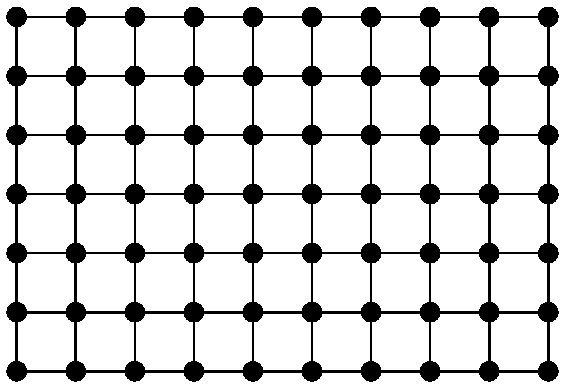
\includegraphics[scale=0.6]{pictures/ctvercovasit.pdf}
  \captionof{figure}{Čtvercová síť o rozměrech $m=7$ a $l=10$ \label{ctvsit}}
}

\paragraph{Jeden řez čtvercové sítě:}

Mějme čtvercovou síť $N = (V,E)$ o rozměrech $n \times n$ a nechť $S_0 \subset V$. Nechť dále vrcholy z množiny $S_0$ leží v síti na jedné přímce a $S_0$ je vrcholovým separátorem sítě $N$, jehož odebráním dojde k rozpadnutí sítě $N$ na dva podgrafy s množinami vrcholů $V_1$ a $V_2$ s pokud možno stejným počtem prvků. Z konstrukce $S$ jsou tyto podgrafy zřejmě také čtvercovými sítěmi. Očíslujme nyní postupně po řádcích vrcholy z množin $V_1$ a $V_2$ a nakonec očíslujme vrcholy $S_0$. Toto očíslování nazýváme jednoúrovňově-dělicím (one-level dissection ordering) a vidíme, že zřejmě splňuje podmínky kladené výše na zobrazení $\varphi$.

\paragraph{Vnořené řezy pro čtvercovou síť: }

Abychom získali očíslování pro metodu vnořených řezů, pokračujeme v dělení komponent s množinami vrcholů $V_1$, $V_2$. Obdobným způsobem jako v prvním kroku vybereme $S_1$, resp. $S_2$ tak, aby byla vhodným vrcholovým separátorem $G(V_1)$, resp. $G(V_2)$. Nyní opět každou část přečíslujeme tak, aby vrcholy v separátoru měly nejvyšší čísla.
Tím se nám podaří docílit toho, že nejen matice sousednosti, ale i její libovolný diagonální blok má tvar (\ref{AG nested}).

\subsection{Dělení obecných grafů metodou vnořených řezů}
\label{NDobecne}

Pro použití metody vnořených řezů pro obecné grafy existují různé přístupy \TODO{cite?}. V této kapitole popíšeme jeden z nich. Jedná se o heuristický algoritmus fungující na principu hledání struktury úrovní daného grafu a následného rozdělení grafu podle úrovně "uprostřed".

Mějme souvislý graf $G=(V,E)$. Algoritmus pro jeho rozdělení využívající metodu vnořených řezů pak vypadá následovně.

\begin{enumerate}
  \item Položíme $W=V$ a $N=|V|$.
  \item \label{forloop} Nalezneme souvislou komponentu $G(C)$ grafu $G(W)$.
  \item Vezmeme libovolný vrchol $v\in C$. Vrchol $v$ je vhodné jej volit tak, aby byl daleko od centra grafu \TODO{dodefinovat centrum!} $G(C)$.
  \item Vytvoříme strukturu úrovní $\mathcal{L}=\{L_0, \ldots ,L_l\}$ grafu $G(C)$ vycházející z vrcholu $v$, tj. rozdělíme množinu vrcholů $C$ grafu $G(C)$ na vzájemně disjunktní množiny $L_1, \ldots, L_l$ definované následovně:
      \begin{align*}
        L_0 & := v \\
        L_i & := \mathrm{adj}_{G(C)}(L_{i-1}) \setminus \bigcup_{k=0}^{i-1} L_k \quad {\rm pro} \ i \in \{2,\ldots,l\}
      \end{align*}
  \item Separátor $S$ grafu $G(C)$ volíme následovně. Pokud $l \leq 2$ položíme separátor roven $C$. Jinak definujeme $j := \floor*{\frac{l+1}{2}}$ a separátor položíme roven
      \[
        S = \left\{y \in L_j \mid \mathrm{adj}_{G(C)}(y) \cap L_{j+1} \neq \emptyset \right\}
      \]
  \item Očíslujeme vrcholy separátoru čísly $N-|S|+1,\ldots,N$
  \item Položíme $W:=W \setminus S$ a $N := N-|S|$.
  \item Pokud $W \neq \emptyset$ vrátíme se na krok \ref{forloop}, jinak skončíme.
\end{enumerate}

%----------------------------------------------------------------------

\chapter{Rozklady matic}

Při řešení maticových úloh velkých rozměrů je často výhodné si danou matici rozložit na součin dvou nebo více matic a díky tomu původní problém převést na sérii výpočetně jednodušších problémů. Jako klasické příklady úloh z numerické lineární algebry, při jejichž řešení nám mohou rozklady matic pomoci, uveďme hledání řešení soustav lineárních algebraických rovnic či problém nalezení vlastních či singulárních čísel a příslušných vektorů. Rozklady matic navíc hrají nezanedbatelnou roli například v QR algoritmu, LR algoritmu \cite{govl:83} nebo Lanczosově algoritmu \cite{lanc:50,paig:72}. Rozklady matic nám mohou pomoci odhalit i teoretické vlastnosti a strukturu matic a odpovídajících maticových problémů. Příkladem takového rozkladu je singulární rozklad (SVD decomposition) \cite{govl:83}.

Rozklady matic můžeme rozdělit na dvě základní skupiny - úplné rozklady a neúplné rozklady. Úplné rozklady dokážou nalézt z teoretického hlediska přesný výsledek v konečně mnoha krocích. Naopak neúplné rozklady jsou iterativními metodami, tj. algoritmy, které získávají v každém svém kroku přesnější aproximaci řešení s použitím výsledku předchozí aproximace a k přesnému výsledku konvergují. Pro získání celkového řešení soustavy je pak třeba je kombinovat s nějakou iterační metodou \cite{temp94}. Vzhledem k našemu cíli zkoumat Choleského rozklad, jakožto zástupce úplných rozkladů, se v dalším textu nebudeme neúplnými rozklady hlouběji zabývat. 

V této práci nás budou zajímat především rozklady, které se týkají řídkých matic, tedy matic, které obsahují velké množství nulových prvků. U takových matic bereme pro zefektivnění výpočtů do úvahy strukturu jejich nenulových prvků. Při výpočtu úplného rozkladu řídké matice může v průběhu rozkladu docházet ke změnám ve struktuře jejích nenulových prvků. Proces výpočtu úplného rozkladu může být pak výpočetně velmi náročný \TODO{cite}.

V námi popisovaném základním modelu rozkladů matic se omezíme na úplný rozklad symetrické a pozitivně definitní matice. Nejedná se o samoúčelné omezení, při řešení mnoha praktických úloh se setkáváme právě s maticemi splňujícími tyto podmínky. Navíc se ukazuje, že i pro matice, které nejsou symetrické nebo pozitivně definitní, lze při jejich rozkladech vyjít z tohoto modelu. \TODO{cite}

\section{Úplné rozklady}

Společným znakem algoritmů pro úplný rozklad matice je, že při práci v přesné aritmetice dokážou tyto algoritmy najít přesný rozklad matice v konečně mnoha krocích. Nejklasičtějším příkladem takovéhoto algoritmu je symetrická eliminace, jejímž speciálním případem je Choleského rozklad, který pro nás bude obzvláště zajímavý. V této kapitole nebudeme ve schématech rozlišovat řídké a husté matice.

\subsection{Symetrická eliminace}

Cílem \textbf{symetrické eliminace} je rozložit danou čtvercovou matici $A$ na tvar $LDL^T$, kde $L$ je dolní trojúhelníková matice a $D$ je diagonální matice. Obecně pro indefinitní matice je třeba pro zajištění numerické stability tohoto algoritmu vynásobit danou matici nějakou permutační maticí \cite{fomo:67}. Pro pozitivně definitní matice je však stabilita zajištěna i bez toho \cite{wil:68}.

Mějme matici $A$ o rozměrech $N \times N$. Symetrickou eliminací matice $A$ nazveme hledání konečných posloupností $(A_j)_{j=0}^{N-1}$, $(L_j)_{j=1}^{N-1}$ splňujících, že $\left(\forall i \in \{1,...,N-1\}\right)\left(A_{i-1}=L_i A_i L_i^T \right)$ a $A_{N-1}=D$.
Předpis pro hledání těchto posloupností je následující:

\begin{gather}
\begin{aligned}
\label{SymEl}
A_0 & = A = \left( \begin{matrix}
               d_1 & v_1^T \\
               v_1 & \bar{H}_1
             \end{matrix} \right)
           =\left(\begin{matrix}
              1               & 0 \\
              \frac{v_1}{d_1} & I_{N-1}
            \end{matrix} \right)
            \left(\begin{matrix}
              d_1 & 0 \\
              0   & \bar{H}_1-\frac{v_1v_1^T}{d_1}
            \end{matrix} \right)
            \left(\begin{matrix}
              1 & \frac{v_1^T}{d_1} \\
              0 & I_{N-1}
            \end{matrix} \right) \\
    &     = L_1
            \left(\begin{matrix}
              d_1 & 0 \\
              0 & H_1
            \end{matrix} \right)
            L_1^T
          = L_1 A_1 L_1^T \\
  A_1 & = \left( \begin{matrix}
               d_1 &  0   & 0 \\
               0   &  d_2 & v_2^T \\
               0   &  v_2 & \bar{H}_2
             \end{matrix} \right)
        =  L_2 A_2 L_2^T \\
    & \vdots \\
  A_{N-1} & = D,
\end{aligned}
\end{gather}

kde $H_i=\bar{H}_i-\frac{v_i v_i^T}{d_i}$.
Zřejmě pak $A = LDL^T$, kde $L:=L_1\cdots L_{N-1}$.

\subsection{Choleského rozklad}
\label{CholeskyChapter}
\textbf{Choleského rozklad} je speciálním případem symetrické eliminace. Jeho cílem je rozložit pozitivně definitní matici $A$ na tvar $A=LL^T$, kde matici $L$ označujeme jako Choleského faktor matice $A$. Jinými slovy se jedná o symetrickou eliminaci matice $A$, kde požadujeme, aby matice $D$ byla rovna jednotkové matici. Z praktického hlediska jde o modifikaci Gaussovy eliminační metody pro symetrické pozitivně definitní matice. Základní informaci o existenci Choleského rozkladu pozitivně definitní matice nám dává následující věta, jejíž důkaz můžeme nalézt například v \cite{govl:83}.

\begin{theorem}
  Pro libovolnou pozitivně definitní matici $A$ existuje jednoznačný rozklad $A=LL^T$, kde L je dolní trojúhelníková matice s kladnými prvky na diagonále.
\end{theorem}

Pro výpočet Choleského rozkladu matice $A$ stačí modifikovat algoritmus \ref{SymEl} tak, aby matice $D$ vznikající při symetrické eliminaci matice $A$ byla rovná jednotkové matici. Toho dosáhneme následovně:

\begin{gather}
\begin{aligned}
\label{Cholesky}
A_0 & = A = \left( \begin{matrix}
               d_1 & v_1^T \\
               v_1 & \bar{H}_1
             \end{matrix} \right)
           =\left(\begin{matrix}
              \sqrt{d_1}      & 0 \\
              \frac{v_1}{\sqrt{d_1}} & I_{N-1}
            \end{matrix} \right)
            \left(\begin{matrix}
              1   & 0 \\
              0   & \bar{H}_1-\frac{v_1v_1^T}{d_1}
            \end{matrix} \right)
            \left(\begin{matrix}
              \sqrt{d_1} & \frac{v_1^T}{\sqrt{d_1}} \\
              0 & I_{N-1}
            \end{matrix} \right) \\
    &     = L_1
            \left(\begin{matrix}
              1 & 0 \\
              0 & H_1
            \end{matrix} \right)
            L_1^T
          = L_1 A_1 L_1^T \\
  A_1 & = \left( \begin{matrix}
               1   &  0   & 0 \\
               0   &  d_2 & v_2^T \\
               0   &  v_2 & \bar{H}_2
             \end{matrix} \right)
        =  L_2 A_2 L_2^T \\
    & \vdots \\
  A_{N-1} & = L_N I_N L_N^T,
\end{aligned}
\end{gather}

kde opět zřejmě platí, že $L=L_1...L_N$.

\medskip

Matici $L$ můžeme však z matic $L_1,\ldots,L_N$ vypočítat výrazně jednodušším způsobem.

\begin{lemma}
\label{Lsoucet}
    Při konstrukci Choleského rozkladu $LL^T$ matice $A$ pomocí algoritmu (\ref{Cholesky}) platí
    \begin{equation}
      L = L_1 + L_2 + \ldots + L_N - (N-1)I_N,
    \end{equation}
    tj. $i$-tý sloupec $L$ je roven $i$-tému sloupci $L_i$.
\end{lemma}
\begin{proof}
  Matice $L_i$ má tvar
  \[
  \left(
  \begin{matrix}
    1 &        &   &                              &   &        &   \\
      & \ddots &   &                              &   & 0      &   \\
      &        & 1 &                              &   &        &   \\
      &        &   & \sqrt{d_i}                   &   &        &   \\
      &        &   & \frac{\vec{v_i}}{\sqrt{d_i}} & 1 &        &   \\
      & 0      &   &                              &   & \ddots &   \\
      &        &   &                              &   &        & 1
  \end{matrix}
  \right).
  \]
  Vynásobením matic $L_i$ a $L_j$, kde $i < j$, zjevně dostanu
  \[
  \left(
  \begin{matrix}
    1 &        &   &                              &   &        &   \\
      & \ddots &   &                              &   & 0      &   \\
      &        & \sqrt{d_i} &     &   &        &   \\
      &        & \frac{\vec{v_i}}{\sqrt{d_i}}  &     \ddots               &   &        &   \\
      &        &   &  & \sqrt{d_j} &        &   \\
      & 0      &   &  & \frac{\vec{v_j}}{\sqrt{d_j}}  & \ddots &   \\
      &        &   &  &   &        & 1
  \end{matrix}
  \right),
  \]
  což je přesně matice $L_i + L_j - I$.
  Z toho již plyne tvrzení lemmatu.
\end{proof}

Pro výpočet prvků matice $L$ existují tři základní postupy: submaticové schéma vyplývající přímo z lemmatu \ref{Lsoucet}, řádkové schéma s použitím metody ohraničování a sloupcové schéma. V přesné aritmetice jsou všechna tři tato schémata ekvivalentní, ale v případě aritmetiky v konečné přesnosti, se kterou se standardně při počítačových výpočtech setkáváme, můžou schémata dávat různé výsledky. Tato schémata napočítávají prvky matice $L$ v různém pořadí.

\paragraph{Submaticové schéma}
S pomocí lemmatu \ref{Lsoucet} můžeme navrhnout submaticové schéma pro výpočet faktoru $L$ následovně. Matici $L$ získáváme po sloupcích, ale při výpočtu $i$-tého sloupce zároveň počítáme submatici $H_i = \bar{H}_i-\frac{v_i v_i^T}{d_i}$ matice $A$, kterou potřebujeme pro výpočet zbylých částí faktoru matice $A$ (viz algoritmus (\ref{Cholesky})).

\paragraph{Řádkové schéma - metoda ohraničování}
Jiným přístupem, který můžeme zvolit pro získání Choleského rozkladu $L L^T$ matice $A$ je řádkové schéma využívající metodu ohraničování (bordering method) \cite{fad:59, ort:88}. Nejprve přepišme matici $A$ do tvaru
\[
A =
\begin{pmatrix}
  M & \vec{u} \\
  \vec{u^T} & s
\end{pmatrix},
\]
přičemž pro odvození vztahu pro výpočet prvků faktoru $L$ předpokládejme, že Choleského rozklad $L_M L_M^T$ matice $M$ již známe. Pak pro Choleského rozklad matice $A$ platí:
\[
A =
\begin{pmatrix}
  L_M & 0 \\
  \vec{w}^T & t
\end{pmatrix}
\begin{pmatrix}
  L_M^T & \vec{w} \\
  0 & t
\end{pmatrix},
\]
kde je zřejmě $\vec{w}=L_M^{-1}\vec{u}$ a $t=(s-\vec{w}^T\vec{w})^{1/2}$.

Pro získání Choleského rozkladu matice $M$, jehož znalost jsme výše předpokládali, můžeme použít stejný postup. Rekurzivním použitím této metody dostáváme soustavu lineárních algebraických rovnic pro výpočet $i$-tého řádku matice $L$, kde $l_{i,j}$ značí $(i,j)$-tý prvek matice $L$.
\begin{gather*}
\begin{pmatrix}
  l_{1,1} &  & 0 \\
  \vdots  & \ddots &  \\
  l_{i-1,1} & \cdots & l_{i-1,i-1}
\end{pmatrix}
\begin{pmatrix}
  l_{i,1} \\
  \vdots \\
  l_{i,i-1}
\end{pmatrix}
=
\begin{pmatrix}
  a_{i,1} \\
  \vdots \\
  a_{i,i-1}
\end{pmatrix} \\
 l_{i,i} = \left(a_{i,i} - \sum_{j=1}^{i-1}{l_{i,j}^2}\right)^\frac12.
\end{gather*}

\paragraph{Sloupcové schéma}
Jedná se o obdobný postup jako v řádkovém schématu, pouze napočítáváme prvky matice $L$ po sloupcích. Vzorce, které nám pro výpočet prvků matice $L$ vzniknou jsou pro $j = 1,2,\ldots, N$ a pro $i = j+1,j+2,\ldots,N$ následující:
\begin{align*}
  l_{j,j} &= \left(a_{j,j} - \sum_{k=1}^{j-1}{l_{j,k}^2}\right)^\frac12 \\
  l_{i,j} &= \left(a_{i,j} - \sum_{k=1}^{j-1}{l_{i,k}l_{j,k}}\right)/l_{j,j}.
\end{align*}

\subsubsection{Choleského rozklad řídkých matic}
\label{Choleskysparse}

V praktických aplikacích Choleského rozkladu se často setkáváme s řídkými maticemi, navíc jsou pro nás řídké matice zajímavé i z hlediska dělení příslušných grafů. Pokud máme řídkou matici, v optimálním případě bychom chtěli, aby i její Choleského faktor byl řídká matice, jejíž dolní trojúhelník má stejnou strukturu jako dolní trojúhelník původní matice.

Mějme čtvercovou matici $A$ o rozměrech $N\times N$ a její Choleského rozklad $LL^T$. Základním problémem výše zmíněných algoritmů je, že matice $L$ běžně obsahuje nenulové prvky na místech, na nichž měla matice $A$ nuly. Toto zaplňování je způsobeno při vytváření posloupnosti matic $H_i$ (viz algoritmus \ref{Cholesky}), konkrétně při přechodu od matice $\bar{H}_i$ k matici $H_i$. Připomeňme, že mezi těmito dvěma maticemi platí vztah
\[
H_i = \bar{H}_i - \frac{\vec{v_i}\vec{v_i}^T}{d_i}.
\]
Označme $\eta(A)$, resp. $\eta(\vec{v})$ počet nenulových prvků matice $A$, resp. vektoru $v$. Pak z lemmatu \ref{Lsoucet} a ze vztahu pro výpočet $L_i$ v Choleského algoritmu \ref{Cholesky} zřejmě platí
\[
\eta(L) = N + \sum_{i=1}^{N-1}\eta(\vec{v_i}).
\]
Vyslovme větu, ze které nám vyplyne počet informaci o počtu multiplikativních operací (násobení a dělení) potřebných pro pro výpočet Choleského rozkladu matice $A$.
\begin{theorem}
\label{Cholesky_operace}
  Počet multiplikativních operací potřebných pro výpočet Choleského rozkladu $LL^T$ matice $A$ o rozměrech $N \times N$ je roven
  \[
  \frac12\sum_{i=1}^{N-1}\eta(v_i)\left(\eta(v_i)+3\right)=
  \frac12\sum_{i=1}^{N-1}\left(\eta(L_{*i})-1\right)\left(\eta(L_{*i})+2\right),
  \]
  kde $L_{*i}$ označuje $i$-tý sloupec matice $L$.
\end{theorem}
\begin{proof}
  Jednotlivá schémata pro výpočet matice $L$ popsaná v předchozí kapitole se liší pouze v pořadí, v němž výpočet prvků matice $L$ provádějí.

  V $i$-tém kroku algoritmu potřebujeme $\eta(\vec{v_i})$ operací pro výpočet $v_i/\sqrt{d_i}$ a $\frac12\eta(\vec{v_i})\left(\eta(\vec{v_i})+1\right)$ operací pro vytvoření matice $\frac{\vec{v_i}\vec{v_i}^T}{d_i}$. Tvrzení věty dostaneme sečtením přes všechna $i$.
\end{proof}

\begin{remark}
Pro hustou matici $B$ platí, že počet nenulových prvků v jejím Choleského faktoru $L_B$ je roven $\frac12 N(N+1)$.
Z věty \ref{Cholesky_operace} je tedy počet operací potřebný pro výpočet Choleského rozkladu matice $B$ roven
\begin{equation}\label{pocetoperaci}
  \frac12 \sum_{1}^{N-1}i(i+3) = \frac16 N^3 + \frac12 N^2 - \frac23 N.
\end{equation}
Z toho plyne, že počet operací pro výpočet Choleského rozkladu libovolné řídké matice o rozměrech $N \times N $ lze seshora odhadnout číslem daným vztahem (\ref{pocetoperaci}).
\end{remark}

Problém zaplňování se dá alespoň částečně vyřešit tím, že místo rozkladu matice $A$ provádíme rozklad matice $PAP^T$, kde $P$ je nějaká permutační matice (tj. matice, kterou když vynásobíme matici $A$, dojde pouze k permutaci řádků, resp. sloupců matice $A$). Vzhledem k tomu, že jsme od začátku předpokládali, že je matice $A$ symetrická a pozitivně definitní, je i matice $PAP^T$ symetrická a pozitivně definitní. Pokud máme zadán problém řešení soustavy $Ax=b$, převedeme jej na problém řešení soustavy $(PAP^T)(Px)=Pb$. Tento problém je úzce spjat s problémem očíslování grafů při jejich dělení a budeme se jím zabývat v dalších kapitolách.

%----------------------------------------------------------------------

\chapter{Další parametry pro dělení grafu}
\label{dalsiParametry}

Dělení grafu lze využít jako nástroj pro paralelizaci problémů, které lze převést na úlohy na grafech. Jedním z takových problémů je problém minimalizace zaplnění v Choleského faktoru dané matice pomocí permutace řádků a sloupců popsaný v kapitole \ref{Choleskysparse}, který lze vzhledem ke vztahu matic a grafů popsanému výše v kapitole \ref{GrMatRel} převést na problém dělení odpovídajícího grafu.

Jak bylo zmíněno, při dělení grafu podle klasické definice bereme ohled pouze na dvě kritéria: na velikost separátoru a vyváženost jednotlivých částí rozdělení. V případě, že dělení grafu využíváme jako součást komplexnějšího algoritmu, například pro paralelizaci nějaké maticové úlohy, nemusí být rozdělení vytvořené s ohledem na tato kritéria optimální. V takovém případě je nutné brát ohled na to, jaké operace budeme na výsledných podgrafech provádět a v závislosti na tom specifikovat nová kritéria. Pro dělení grafu s ohledem na více než dvě základní kritéria popsaná výše existují dva základní přístupy. Můžeme hledat rozdělení grafu optimalizující všechna kritéria zároveň (apriorní přístup), nebo můžeme graf rozdělit pomocí některého ze základních algoritmů pro dělení grafu a poté vzniklé rozdělení vylepšit tak, abychom optimalizovali vyváženost operací (aposteriorní přístup).

V této práci se zaměříme na situaci, kdy je dělení grafů použito jako nástroj pro vyvažování počtu operací na jednotlivých oblastech při paralelizaci Choleského rozkladu. Požadujeme tedy, aby počet operací potřebný pro Choleského rozklad na jednotlivých oblastech byl v optimálním případě stejný a zároveň co nejmenší. Zřejmě nám takto vzniká kritérium, které není zahrnuto v kritériích podle klasické definice - ta totiž neberou v potaz hustotu hran v podgrafech vzniklých dělením původního grafu, neboli v řeči matic počet nenulových prvků matic sousednosti jednotlivých podgrafů. Počet operací potřebných pro vypočítání rozkladu na jednotlivých oblastech může být kvůli tomu výrazně odlišný. Námi navržený algoritmus bude využívat aposteriorního přístupu, nejprve tedy nalezneme suboptimální řešení vzhledem k základním kritériím a poté budeme hledat vhodné očíslování vrcholů daných podgrafů a přesouvat vrcholy mezi jednotlivými částmi rozdělení s cílem vylepšit jej vzhledem k Choleského rozkladu.

Mějme graf $G$ a jeho rozdělení na podgrafy $G_1, \ldots, G_k$ s maticemi sousednosti $A_{G_1}, \ldots, A_{G_k}$. Provedeme Choleského rozklad matic $A_{G_1}$, $A_{G_2}$, označme
\[
  A_{G_i} = L_{G_i}L_{G_i}^T \ {\rm pro} \ i = 1,2.
\]
Pokud existují $i,j \in \{1,\ldots,k \}$ tak, že matice $L_{G_i}^T$ a $L_{G_j}^T$ budou mít výrazně různý počet nenulových prvků, je zřejmé, že toto rozdělení grafu $G$ je nevhodné pro napočítávání Choleského rozkladu na oblastech vzhledem k vyváženosti na počet operací. Někdy pro vyvážení rozdělení za účelem Choleského rozkladu na oblastech stačí vhodně přečíslovat vrcholy podgrafů $G_1, \ldots, G_k$ a tím změnit matice sousednosti odpovídající jednotlivým podgrafům.

\begin{remark}
Mějme soustavu lineárních algebraických rovnic $Ax=b$ a hledejme její řešení pomocí Choleského rozkladu této matice $A=LL^T$ za pomoci dělení grafů. Pro vyřešení soustavy potřebujeme vyřešit rovnice
\begin{align*}
  Ly =& b \\
  L^Tx= & y
\end{align*}
Pokud rozdělíme graf příslušný matici $A$ na $k$ částí a provedeme rozklad matic $A_1=L_1 L_1^T, \ldots, A_k=L_k L_k^T$ odpovídajících vzniklým podgrafům a matice $A_S=L_S L_S^T$ odpovídající vrcholovému separátoru, pak lze soustavu $Ly=b$ napsat ve tvaru
\[
\begin{pmatrix}
  L_1 &     &        &      & \\
      & L_2 &        &      & \\
      &     & \ddots &      & \\
      &     &        & L_k  & \\
  S_1 & S_2 &        & S_k  & L_S
\end{pmatrix}
\begin{pmatrix}
  y_1 \\
  y_2 \\
  \vdots \\
  y_k \\
  y_S
\end{pmatrix}
=
\begin{pmatrix}
  b_1 \\
  b_2 \\
  \vdots \\
  b_k \\
  b_S
\end{pmatrix}
\]
a tedy
\begin{align*}
  y_1= & L_1^{-1}b_1 \\
  y_2= & L_2^{-1}b_2 \\
  \vdots \\
  y_k= & L_k^{-1}b_k \\
  y_S= & L_1^{-1}(b_S - S_1 y_1 - S_2 y_2 - \ldots - S_k y_k)
\end{align*}
Je vidět, že zatímco výpočet $y_1, \ldots, y_k$ může probíhat paralelně, výpočet $y_S$ je závislý na $y_1, \ldots, y_k$. Je tedy vhodné, aby vrcholový separátor byl malý.


Soustavu $L^Tx=y$ poté vyřešíme obdobně.
\end{remark}

\medskip

Jak vidíme, vyvstávají nám při dělení grafu s cílem vypočítávat Choleského rozklad na oblastech dvě základní otázky:
\begin{enumerate}
  \item Jak najít očíslování grafu takové, aby Choleského rozklad na jednotlivých podgrafech byl vyvážený?
  \item Jak určit počet nenulových prvků v Choleského rozkladu matice se strukturou matice sousednosti jednotlivých podgrafů?
\end{enumerate}
Způsob hledání odpovědí na tyto dvě otázky popíšeme v následujících dvou oddílech.

\section{Algoritmy pro očíslování vrcholů grafu}
\label{Numbering}
V tomto oddíle popíšeme základní algoritmy pro očíslování vrcholů grafu. Zřejmě platí, že přečíslování vrcholů grafu odpovídá permutaci řádků a sloupů v jeho matici sousednosti. Hlavní motivací, proč je pro nás číslování vrcholů grafu důležité, tedy je, že permutací řádků matice můžeme výrazně redukovat počet operací potřebných pro její Choleského rozklad.

Na závěr kapitoly se zmíníme o topologickém číslování vrcholů stromu, které pro nás bude potřebné při popisu eliminačních stromů v kapitole \ref{eltreeChapter}.

\subsection{Číslování vrcholů grafu v závislosti na vzdálenosti od separátoru}
\label{sepDistOrdering}

V této podkapitole popíšeme nejjednodušší metodu číslování vrcholů podgrafu, který vznikl rozdělením původního grafu na $n$ částí.
Tuto metodu lze používat samostatně, ale vzhledem k její povaze ji lze využít i pro vylepšení ostatních metod očíslování grafu,
například ji lze kombinovat s metodou minimálního stupně.

Mějme graf $G = (V,E)$ a jeho vrcholový separátor $G_S$, jehož odebráním se graf rozpadne na $k$ podgrafů $G_1, \ldots, G_k$.
Popišme číslování vrcholů podgrafu $G_i$:

\begin{enumerate}
  \item Položme $\texttt{j := 1}$.
  \item \label{sepDistAlg2} Nalezneme neočíslovaný vrchol $v$ grafu $G_i$ takový, že jeho vzdálenost od vrcholového separátoru v grafu $G$ je maximální.
  \item Tomuto vrcholu dáme číslo $\texttt{j}$, položíme $\texttt{j := j + 1}$.
  \item Pokud jsou všechny vrcholy očíslovány, skončíme, jinak se vrátíme na krok \ref{sepDistAlg2}
\end{enumerate}

Z algoritmu je vidět, že výsledné očíslování vrcholů grafu nemusí být jednoznačné, protože pokud nalezneme dva nebo více vrcholů, jejichž vzdálenost od separátoru je shodná, můžeme je očíslovat v libovolném pořadí.

\subsection{Číslování vrcholů pomocí metody minimálního stupně}
\label{MDordering}
Metoda minimálního stupně je jednoduchým algoritmem pro nalezení očíslování grafu. Algoritmus pro hledání očíslování grafu pomocí této metody je následující:

\begin{enumerate}
  \item Mějme graf $G=(V,E)$ a položme $j:=1$.
  \item \label{mindegloop}
      Nalezneme neočíslovaný vrchol $v$ grafu $G$ s nejmenším stupněm a přiřadíme mu číslo $j$.
  \item Přidáme hrany mezi vrcholy z $\mathrm{adj}_G(v)$ tak, aby $\mathrm{adj}_G(v)$ byla klika v grafu $G$.
  \item Pokud nejsou všechny vrcholy očíslované, zvětšíme $j$ o $1$ a vrátíme se na krok \ref{mindegloop}.
\end{enumerate}

Očíslování vrcholů grafu G pomocí tohoto algoritmu není jednoznačné, protože vrcholů s minimálním stupněm může být více.

\subsection{Smíšené číslování}
Vzhledem k povaze číslování popsaných v oddílech \ref{MDordering} a \ref{sepDistOrdering} můžeme tyto algoritmy zkombinovat. V tomto oddíle popisujeme dvě možnosti přístupu k tomuto problému.

Pokud máme rozdělení $G_1, \ldots, G_k$ grafu $G$ s vrcholovým separátorem $G_S$, můžeme pro očíslování části $G_i$ použít číslování vrcholů pomocí metody minimálního stupně, kde při výběru vrcholu ve \ref{mindegloop}. kroku přidáme kritérium vzdálenosti od separátoru popsané v \ref{sepDistOrdering}. Nejprve tedy nalezneme množinu všech vrcholů grafu $G$, které mají minimální stupeň a poté mezi nimi zvolíme ten, který má nejmenší stupeň.

\TODO{smíšené s různými koef.}

\subsection{Topologické číslování vrcholů stromu}
Topologické číslování vrcholů stromu je intuitivní způsob pro očíslování vrcholů grafu, který je stromem.
\begin{definition}
    Mějme graf $G = (V,E)$, který je stromem. Očíslování jeho vrcholů nazveme topologickým právě tehdy,
    když pro každý vrchol $v \in V$ platí, že libovolný následník vrcholu $v$ ve stromu $G$ má nižší číslo než vrchol $v$.
\end{definition}


\section{Eliminační stromy}
\label{eltreeChapter}
\TODO{Udelat poradek s $[A],[L],a,l$}

V této kapitole se budeme zabývat eliminačními stromy a jejich významem pro rozklady řídkých matic \cite{liu:86,liu:90}. Eliminační stromy při rozkladu matic hrají důležitou roli, protože nám dávají informaci o zaplnění v Choleského faktoru matice bez toho, abychom museli počítat jednotlivé numerické hodnoty. Lze tedy díky nim jednoduše porovnávat vhodnost zvoleného uspořádání řádků a sloupců matice pro Choleského rozklad.

V této kapitole bez újmy na obecnosti předpokládáme, že matice, jejíž Choleského rozklad chceme napočítávat, je ireducibilní, a tedy graf odpovídající této matici je souvislý.

\subsection{Definice eliminačního stromu matice}

Nejprve se omezme na ireducibilní, pozitivně definitní, symetrickou matici $A_T$ o rozměrech $n \times n$, jejíž přidružený graf $G(A_T)$ je kořenový strom. Aby při Choleského rozkladu matice $A_T$ nedošlo k žádnému zaplnění, stačí když pomocí topologického číslování očíslujeme vrcholy jí přidruženého grafu (z předpokladu se jedná o strom) a řádky a sloupce matice $A_T$ seřadíme odpovídajícím způsobem. Pak zjevně platí, že matice $A_T$ má, s výjimkou posledního řádku, pod diagonálou vždy právě jeden nenulový prvek. Díky této vlastnosti označujeme $A_T$ jako perfektní eliminační matici, tj. existuje permutační matice $P$ taková, že Choleského rozklad matice $PA_TP^T$ nebude obsahovat žádné zaplnění \cite{rose:72} (Matici $PA_TP^T$ můžeme vnímat pouze jako přečíslování řádků a sloupců matice $A_T$). 

Proto pro matici $A_T$ můžeme definovat funkci $\texttt{PARENT}:\{1,\ldots,n\} \rightarrow \{1,\ldots,n\}$ následovně:
\begin{align*}
  \forall j \in \{1,\ldots,n-1\} \quad \texttt{PARENT}[j] & := p \quad \Leftrightarrow \quad a_{p,j} \neq 0 \ \wedge \ p > j \\
  \text{a speciálně:} \quad \texttt{PARENT}[n] & := 0.
\end{align*}
Zřejmě ve stromu přidruženém k matici $A_T$ platí, že předchůdcem vrcholu $x_j$ je vrchol $x_{\texttt{PARENT}[j]}$.

Většinou však nepracujeme s maticemi, jejichž přidružený graf by byl stromem. Zobecněme tedy výše popsanou konstrukci pro libovolnou řídkou, ireducibilní, pozitivně definitní, symetrickou matici $A$ o rozměrech $n \times n$. Předpokládejme, že známe Choleského rozklad této matice, tj. $A = LL^T$. \textbf{Maticí se zaplněním} nazveme matici $F$ definovanou jako $F = L + L^T$. Dále zavedeme matice $L_t$ a $F_t$ následovně: $L_t$ je matice vzniklá z $L$ tím, že v každém sloupci vynulujeme všechny prvky pod diagonálou
kromě prvku s nejnižším řádkovým indexem a $F_t := L_t + L_t^T$.

Z definice $F_t$ vidíme, že se jedná o matici, jejíž přidružený graf $G(F_t)$ je strom. Díky tomu můžeme vyslovit následující definici.

\begin{definition}
    \textbf{Eliminačním stromem} matice $A$ nazveme graf $G(F_t)$ popsaný výše, značíme $T(A)$.
    Podstrom eliminačního stromu $T(A)$ s kořenem $x_j$ značíme $T[x_j]$. Množinu vrcholů tohoto stromu značíme taktéž $T[x_j]$.
\end{definition}

Díky této definici můžeme definici funkce $\texttt{PARENT}$ přirozeně rozšířit na matici $A$ následovně:
\[
    \texttt{PARENT}[j] := \min \left\{ i > j \ | \ l_{i,j} \neq 0\right\},
\]
kde $l_{i,j}$ označuje $i,j$-tý prvek matice $L$.

\begin{observation}
Přímo z definice plyne, že $T(A)$ a $T(F)$ jsou identické.
\end{observation}

\begin{observation}
Pokud $x_i$ je vlastním předchůdcem $x_j$ v eliminačním stromu, pak $i > j$.
\end{observation}

\begin{proposition}
  \label{ColDepProposition}
  Nechť $A$ je řídká, ireducibilní, pozitivně definitní, symetrická matice o rozměrech $n \times n$ s Choleského rozkladem $LL^T$ a nechť $i,j \in \left\{1,\ldots,n \right\}$, $i > j$. Pak numerické hodnoty sloupce $L_{\bullet i}$ závisí na sloupci $L_{\bullet j}$ právě tehdy,
  když $l_{i,j} \neq 0$.
\end{proposition}
\begin{proof}
  Tvrzení plyne přímo ze vzorců pro výpočet Choleského rozkladu pomocí sloupcového algoritmu popsaného v kapitole \ref{CholeskyChapter}
\end{proof}

Přímým důsledkem tvrzení \ref{ColDepProposition} je, že graf $G(F)$ zachycuje informace o závislostech mezi jednotlivými sloupci při výpočtu Choleského rozkladu. 

\subsection{Eliminační stromy a Choleského rozklad}
Z definice eliminačních stromů je zřejmé, že budou obsahovat velké množství informací o rozkladu matice a procesu jeho vytváření. Například v \cite{schr:82} byly popsány vlastnosti eliminačních stromů vzhledem ke Gaussově eliminaci. My však budeme eliminační stromy využívat jako nástroj pro výpočet počtu nenulových prvků v Choleského faktoru matice \cite{liu:90}. Uveďme větu, která dává do souvislosti nenulové prvky v Choleského faktoru a strukturu eliminačního stromu \cite{liu:86}.

\begin{theorem}
  Nechť $A$ je řídká, ireducibilní, pozitivně definitní, symetrická matice o rozměrech $n \times n$ s Choleského rozkladem $LL^T$ a nechť $i,j \in \left\{1,\ldots,n \right\}$. Pak $[L]_{ij} \neq 0$ právě tehdy, když vrchol $v_j$ je v eliminačním stromě následníkem vrcholu $v_k$ takového, že $[A]_{ij} \neq 0$.
\end{theorem}

Tato věta nám dává návod, jak vypočítat počet nenulových prvků v Choleského faktoru. Uveďme algoritmus popsaný v \cite{liu:90}, který nám dává návod, jak napočítat počty nenulových prvků v jednotlivých řádcích a sloupcích Choleského faktoru. Obdobný algoritmus s důrazem na implementaci na multiprocesorech můžeme nalézt v \cite{zmgi:88}. Námi popsaný algoritmus je poměrně jednoduchý, efektivnější ale složitější algoritmus pro výpočet počtu nenulových prvků můžeme najít v \cite{gil:94}. Dále v \cite{basm:87} můžeme najít postup, jakým napočítávat počet nenulových prvků ve faktoru a strukturu eliminačního stromu současně.

V uvedeném algoritmu \ref{nonzerosAlgorithm} je použit pracovní vektor \Marker, který složí k označování vrcholů eliminačního stromu, které byly v dané iteraci již uvažovány - indexování vrcholů eliminačního stromu uvažujeme tak, že odpovídá vstupní matici. Eliminační strom je popsán pomocí vektoru $\texttt{PARENT}$, který byl zmíněn výše.

\begin{figure}[ht]
  \centering
  \begin{minipage}{.5\linewidth}
    \begin{algorithm}[H]
      \SetAlgoNoLine
      
      \SetKwArray{Parent}{$\texttt{PARENT}$}
      \TODO{Neni to plagiatorstvi?}

      \For{$j:=1$ \KwTo $n$}{
        $\eta(L_{*j}) := 1$\;
      }
      \For{$i:=1$ \KwTo $n$}{
        $\eta(L_{i*}) := 1$\;
        \Marker{$i$} $ := i$\;
        \For{$k:=1$ \KwTo $i-1$}{
          \If{$[A]_{i,k} \neq 0$}{
            $j:= k$\;
            \While{\Marker{$j$} $\neq i$}{
              $\eta(L_{i*}) := \eta(L_{i*}) + 1$\;
              $\eta(L_{*j}) := \eta(L_{*j}) + 1$\;
              \Marker{$j$} $=i$\;
              $j := $\Parent{$j$}\;
            }
          }
        }
      }
    \end{algorithm}
  \end{minipage}
  \captionof{algocf}{Výpočet počtu nenulových prvků z eliminačního stromu (\cite{liu:90}, upraveno) \label{nonzerosAlgorithm}}
\end{figure}

Algoritmus \ref{nonzerosAlgorithm} nám dává návod jak vypočítat počet prvků v jednotlivých řádcích a sloupcích matice. Pokud nás zajímá pouze počet nenulových prvků v celé matici, můžeme počítat pouze počet prvků v řádcích, resp. sloupcích.

Tento algoritmus nám dává odpověď na to, jak zjistit počet nenulových prvků v matici $L$ z eliminačního stromu matice $A$. Pokud bychom eliminační strom vytvářeli přímo z definice, museli bychom vypočítat Choleského rozklad. Proto potřebujeme algoritmus, který nám sestrojí Eliminační strom - tedy vektor $\texttt{PARENT}$ - bez toho.

Uveďme základní algoritmus pro sestrojení eliminačního stromu matice bez výpočtu jejího Choleského rozkladu. Dále popišme jeho vylepšení, které budeme používat v implementaci. Oba algoritmy jsou převzaté z \cite{liu:86}. 

\begin{figure}[ht]
  \centering
  \begin{minipage}{.7\linewidth}
    \begin{algorithm}[H]
      \SetAlgoNoLine
      
      \SetKwArray{Parent}{$\texttt{PARENT}$}

      \For{$i:=1$ \KwTo $n$}{
        \Parent{$i$} $= 0$\;
        \For{$j:=1$ \KwTo $i-1$}{
          \If{$[A]_{i,j} \neq 0$}{
            $r:= j$\;
            \While{\Parent{$r$} $\neq 0$ {\bf and} \Parent{$r$} $\neq i$}{
              $r := $\Parent{$r$}\;
            }
            \If{\Parent{$r$} $== 0$}{
              \Parent{$r$} $:= i$\;
            }
          }
        }
      }
    \end{algorithm}
  \end{minipage}
  \captionof{algocf}{Základní algoritmus pro hledání eliminačního stromu (\cite{liu:86}, upraveno) \label{eltree1Algorithm}}
\end{figure}

Pro zrychlení tohoto algoritmu použijeme pomocný vektor $\texttt{ANCESTOR}$, který nám zkrátí procházení stromu směrem ke kořeni díky tomu, že v něm bude pro každý vrchol zaznamenáván poslední zpracovaný předek daného vrcholu. Algoritmus pak bude vypadat následovně:

\begin{figure}[ht]
  \centering
  \begin{minipage}{.75\linewidth}
    \begin{algorithm}[H]
      \SetAlgoNoLine
      
      \SetKwArray{Parent}{$\texttt{PARENT}$}
      \SetKwArray{Ancestor}{$\texttt{ANCESTOR}$}

      \For{$i:=1$ \KwTo $n$}{
        \Parent{$i$} $= 0$\;
        \Ancestor{$i$} $= 0$\;
        \For{$j:=1$ \KwTo $i-1$}{
          \If{$[A]_{i,j} \neq 0$}{
            $r:= j$\;
            \While{\Ancestor{$r$} $\neq 0$ {\bf and} \Ancestor{$r$} $\neq i$}{
              $t := $\Ancestor{$r$}\;
              $\Ancestor{$r$} := i$\;
              $r := t$\;
            }
            \If{\Ancestor{$r$} $== 0$}{
              \Ancestor{$r$} $:= i$\;
              \Parent{$r$} $:= i$\;
            }
          }
        }
      }
    \end{algorithm}
  \end{minipage}
  \captionof{algocf}{ Vylepšený algoritmus pro hledání eliminačního stromu (\cite{liu:86}, upraveno) \label{eltree2Algorithm}}
\end{figure}


Algoritmus \ref{eltree2Algorithm} má složitost $O(|E|\log_2 n)$ \TODO{slozitost+citace viz liu:86}. Existuje ještě efektivnější verze tohoto algoritmu, kterou můžeme nalézt v \TODO{ cite Tarjan Data structures and network algorithms}.

Algoritmy uvedené v této kapitole jsou popsány tak, aby byly dostatečně názorné. Ve skutečnosti pro řídké matice uložené v CSR formátu (viz \ref{matrixProgReprez}) neprocházíme všechny prvky dané matice, ale pouze nenulové prvky uložené ve struktuře.

%----------------------------------------------------------------------

\chapter{Algoritmizace a implementace}

Cílem programu, který jsme implementovali, je ukázat, že rozdělení grafu získané za pomoci profesionální numerické knihovny pro dělení grafů METIS, nemusí být vyvážené vzhledem k výpočtu Choleského rozkladu na vzniklých oblastech. Dále jsme se pokusili navrhnout a otestovat metodu přerozdělení grafu založenou na přečíslování vrcholů grafu. Cílem navržené metody je zlepšit rozdělení grafu tak, aby počet operací potřebných pro Choleského faktorizaci na jednotlivých oblastem byl pokud možno stejný a nebyl vyšší než maximum z počtu operací při rozdělení počátečním.

\TODO{Fortran, Fortran90, c++}
\TODO{dělení na kolik částí?}

Naši implementaci můžeme rozdělit na několik logických celků. \TODO{doplnit}

\section{Formát a uložení vstupní matice}
V této podkapitole bude popsán vstupní formát matice a způsob její reprezentace v našem programu.
\TODO{Zajímá nás jen struktura}

\subsection{Vstupní formát matice}

Jako základní matice pro testování výsledků našeho programu nám posloužily matice uložené ve formátu RSA v souborech s příponou \texttt{.rsa} nebo \texttt{.rb}. Jako zdroj pro tyto matice jsme použili kolekci \cite{hbcol}.

\TODO{popis HB formátu}

Pro testování jsme dále používali matice vygenerované při jednoduché pětibodové diskretizaci dvojrozměrné Poissonovy rovnice (podprogram \texttt(poisson)) a několik jednoduchých testovacích matic, které jsme si ručně zapsali do souboru \texttt{testing.f90}

\subsection{Reprezentace matice v programu}
\label{matrixProgReprez}

Matice je v našem programu uložena v \textbf{CSR formátu} (compressed sparse row format) \cite{pis:84,saad:94}, který je běžně využívaným formátem sloužícím pro reprezentaci řídkých matic a grafů. 

Mějme řídkou matici $A$ o rozměrech $n \times n$, která obsahuje $n_e$ nenulových prvků. Tuto matici v programu reprezentujeme pomocí tří polí: pole \texttt{ia} o délce $n+1$ a polí \texttt{ja},\texttt{aa} o délce $n_e$. V poli \texttt{ja} na pozicích \texttt{ia($i$)},\ldots,\texttt{ia($i+1$)-1} jsou uloženy sloupcové indexy nenulových prvků na $i$-tém řádku matice $A$, na odpovídajících pozicích v poli \texttt{aa} jsou uloženy numerické hodnoty těchto prvků.

\begin{example}
  \label{CSRexample}
  Mějme následující symetrickou matici
  \[
    \begin{pmatrix}
      0 & 5 & 0 & 3 & 0 \\
      5 & 0 & 9 & 4 & 2 \\
      0 & 9 & 0 & 0 & 0 \\
      3 & 4 & 0 & 0 & 4 \\
      0 & 2 & 0 & 4 & 0
    \end{pmatrix}
  \]
  Pak její reprezentace ve formátu CSR vypadá následovně:
  \begin{verbatim}
    ia = [ 1, 3, 7, 8, 11, 13 ]
    ja = [ 2, 4, 1, 3, 4, 5, 2, 1, 2, 5, 2, 4 ]
    aa = [ 5, 3, 5, 9, 4, 2, 9, 3, 4, 4, 2, 4 ]
  \end{verbatim}
\end{example}

Pokud budeme uvažovat pouze pole \texttt{ia}, \texttt{ja}, je podle teorie popsané v oddíle \ref{GrMatRel} výsledná reprezentace matice $A$ zároveň reprezentací neorientovaného grafu, kterému matice $A$ odpovídá. Pokud tedy nebudeme brát v úvahu hodnoty jednotlivých prvků matice, můžeme při popisu implementace bez újmy na obecnosti pojmy graf a matice zaměňovat.

\begin{example}
  Vezměme matici z příkladu \ref{CSRexample}. Pak graf, který je reprezentován pomocí polí \texttt{ia}, \texttt{ja} je zobrazen na obrázku \ref{MatGrPicture}
\end{example}

\section{Knihovna METIS pro dělení grafu}

Pro samotné dělení grafu na $k$ částí jsme využili knihovnu pro dělení grafů METIS \cite{kary:13} verze 5.1.0. Vzhledem k tomu, že jsme dělení grafů používali jako nástroj pro vyvažování počtu operací při Choleského rozkladu na jednotlivých oblastech, potřebovali jsme nalézt rozdělení grafu pomocí vrcholového separátoru. Takové rozdělení nám poskytne rutina \texttt{METIS\_ComputeVertexSeparator}, kterou jsme ve Fortranu implementovali pomocí rozhraní \texttt{metis\_interface.f95} a \texttt{metisinclude.c}.

Zmíněná rutina není zmíněna v oficiální dokumentaci knihovny METIS a není tedy ve své základní verzi kompatibilní s jazykem Fortran. Proto bylo nutné učinit několik změn ve formátu CSR tak, aby bylo možné rutinu použít. Nejprve bylo třeba odebrat z grafu smyčky a poté jej přečíslovat tak, aby bylo vrcholy indexovány od 0, jak je požadováno v jazycích C a C++.

Výstupem rutiny \texttt{METIS\_ComputeVertexSeparator} je pole $part$ o délce rovné počtu vrcholů grafu. Na $i$-té pozici tohoto pole je číslo od $1$ do $k+1$ (po převedení do Fortranového zápisu), které určuje, ve které části rozdělení se daný vrchol nachází. $k+1$ značí, že daný vrchol je ve vrcholovém separátoru.

\section{Tvorba podgrafů a přerozdělení}
\TODO{doplnit}
\subsection{Číslování}
\TODO{doplnit}
\subsection{Přerozdělení}
\TODO{doplnit}

\section{Výpočet Choleského rozkladu}
\TODO{doplnit}

\section{Softwarové požadavky pro běh}
\TODO{mám to tam vůbec dávat?}
Pro úspěšné slinkování a zkompilování
\TODO{nainstalovaný METIS}

%----------------------------------------------------------------------

\chapter*{Závěr}
\TODO{doplnit}
\TODO{motivace: nelineární problém viz Tumovy stranky}


\newpage

\TODO{udelat poradek v citacich}

\bibliographystyle{plain}
\bibliography{diplomka}

\end{document} 